% !TEX root = ../Dokumentation.tex
\subsection{Gesamtübersicht}

\begin{figure}[h!]%Position festigen
\centering
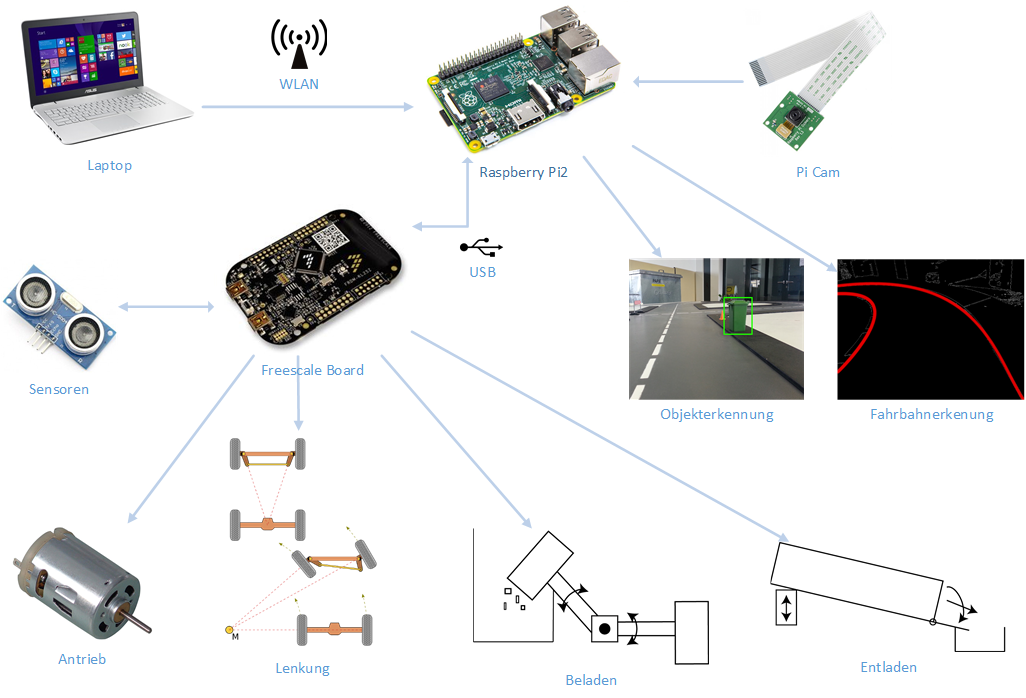
\includegraphics[width=0.9\textwidth]{03_Loesungskonzept/pictures/uebersichtszeichnung.png}
\caption{Übersichtszeichnung}
\label{fig:Java}
\end{figure}

\subsubsection{Zusammenspiel}\\[0.2cm]
Wie die obige Darstellung zeigt, besteht zwischen allen Komponenten ein enges Zusammenspiel.
So wird beispielsweise die gesamte Bilderkennung über den Minicomputer gesteuert. Dieser erhält seine Daten einerseits durch die Kamera, aber auch von den Sensoren welche über den Microcontroller an ihn gesendet werden. Nachdem die Informationen bearbeitet wurden, werden Befehle an den Microcontroller geschickt, welcher die Ansteuerung der Motoren übernimmt. Die Motoren wiederum, lösen die mechanischen Bewegungen aus wie z.B die Schwenkung der Kamera oder das Senken des Greifarmes.\\[0.2cm]
\subsubsection{Schnittstellen}
\begin{figure}[h!]%Position festigen
\centering
\includegraphics[width=0.9\textwidth]{03_Loesungskonzept/pictures/verteilungsdiagramm.png}
\caption{Schnittstellenübersicht}
\label{fig:Java}
\end{figure}
In Abbildung 2 wird eine detaillierte Ansicht der Komponente dargestellt, insbesondere was die Schnittstellen betrifft. So ist erkenntlich, dass der Microcontroller als Hauptknoten fungiert und als Schnittstelle für analoge wie auch digitale Signale dient.
\subsubsection{Geschwindigkeitsregelung}
Damit das Fahrzeug mit einer konstanten Geschwindigkeit fahren kann, muss ein Regler eingebaut werden.
\begin{figure}[H]
	\centering
	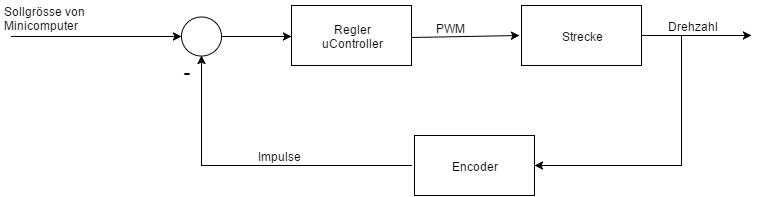
\includegraphics[width=0.5\textwidth]{03_Loesungskonzept/pictures/Gesch_Regelung.png}
	\label{fig:Flex_R_Kennlinie}
	\caption{Grober Regelkreis}
\end{figure}
Hier zu sehen ist der grobe Regelkreis. Der Sollwert wird vom Minicomputer vorgegeben und an das Mikrokontrollerboard weitergeleitet. In diesem wird dann die Regelung implementiert. Der Regelausgang ist ein PWM Signal, der die Geschwindigkeit des Antriebsmotors bestimmt. 
\subsubsection{Lenkregeung}